\chapter{Methodology}
\label{chap:methodology}

This chapter presents the proposed methodology for binary causal question answering over directed causal knowledge graphs. Section~\ref{sec:method_formulation} specifies the graph-based problem setting considered in this work. Section~\ref{sec:method_search} introduces the bounded embedding-guided $A^*$ search procedure, including its traversal cost and heuristic functions. Section~\ref{sec:method_finetuning} motivates the fine-tuning of the embedding space for more effective search guidance. Finally, Section~\ref{sec:method_framework} provides an overview of the main software components and interactive demonstration.

\section{Problem Setting}
\label{sec:method_formulation}

Following the graph-based formulation introduced in Section~\ref{sec:foundations_graphs}, this thesis treats binary causal question answering as directed reachability. Given two concepts $A$ and $B$ with corresponding graph nodes $a,b\in V$, the task is to determine whether a directed path from $a$ to $b$ can be found. A discovered path yields a positive answer, while failure to find one yields a negative answer under the applied search procedure.

\section{Embedding-Guided \texorpdfstring{$A^*$}{A*} Search}
\label{sec:method_search}

To search efficiently for a directed causal path from $a$ to $b$, this work employs an embedding-guided $A^*$ algorithm. In spatial path-finding applications, $A^*$ heuristics often rely on geometric distances, whereas causal knowledge graphs provide no spatial coordinates from which such estimates can be derived. Therefore, each graph node is mapped to a corresponding point in a $d$-dimensional embedding space according to
\[
\phi \colon V \rightarrow \mathbb{R}^{d},
\]
where $\phi(v)$ denotes the vector representation of node $v$. The traversal cost of an edge $(u,v)$ is defined as the distance between the embeddings of $u$ and $v$,
\[
c(u,v)=d\bigl(\phi(u),\phi(v)\bigr),
\]
where $d(\cdot,\cdot)$ denotes either cosine or Euclidean distance. For a node $n$, the accumulated cost from the start node $a$ is defined as
\[
g(n)=\sum_{(u,v)\in P_{a,n}} c(u,v),
\]
where $P_{a,n}$ denotes the currently known path from $a$ to $n$. The heuristic function estimates the remaining distance from $n$ to the target node $b$ as
\[
h(n)=d\bigl(\phi(n),\phi(b)\bigr),
\]
and the priority of each node is determined by
\[
f(n)=g(n)+h(n).
\]
Let $\tau$ denote the maximum visited-node budget, with $\tau=-1$ indicating that no limit is applied. Nodes are expanded in ascending order of $f(n)$ until $b$ is reached, the priority queue is exhausted, or $\tau$ is exceeded. The implementation retains the lowest known path cost for each node and does not reopen nodes after expansion. This reduces traversal overhead but does not retain the optimality guarantee of classical $A^*$ when the heuristic is not consistent. Algorithm~\ref{alg:bounded-astar} presents the proposed bounded embedding-guided $A^*$ search.

\section{Fine-Tuning the Embedding Space}
\label{sec:method_finetuning}

The evaluated pretrained embedding models are designed primarily for semantic similarity, retrieval, or ranking rather than causal graph traversal~\cite{allmpnet:modelcard,bge:modelcard,granite:modelcard,mxbai:modelcard,qwen3:modelcard}. Their original embedding spaces therefore do not necessarily reflect which neighboring nodes are most relevant for reaching a causal target. To improve the search heuristic, the embedding space is fine-tuned using successful causal search paths. At each step, the successor on the discovered path is contrasted with alternative outgoing neighbors, encouraging the model to assign more favorable embedding-space distances to transitions that lead toward the target. The resulting representations are therefore better aligned with the requirements of embedding-guided $A^*$ search. Chapter~\ref{chap:train} details this procedure.

\section{Implementation Overview}
\label{sec:method_framework}

The implementation covers graph search, hyperparameter optimization, model training, evaluation, and interactive visualization. Dataset processing relies on Hugging Face Datasets~\cite{lhoest:2021}, while Optuna~\cite{akiba:2019} is used to optimize the hyperparameters before training. The Sentence Transformer models~\cite{reimers:2019} are subsequently trained with PyTorch~\cite{paszke:2019} and PyTorch Lightning~\cite{falcon:2019}, while NumPy~\cite{harris:2020} is used for embedding storage and access. The demonstration shown in Figure~\ref{fig:frontend-demo} is implemented using FastAPI~\cite{ramirez:fastapi} and 3d-force-graph~\cite{asturiano:3dforcegraph}. It allows users to select a graph, embedding model, and Matryoshka dimension, execute embedding-guided $A^*$ search, and visualize the resulting causal path.\footnote{The demonstration is deployed at \url{https://pathfinding.demo.causenet.org}.}

\begin{figure}[t]
    \centering
    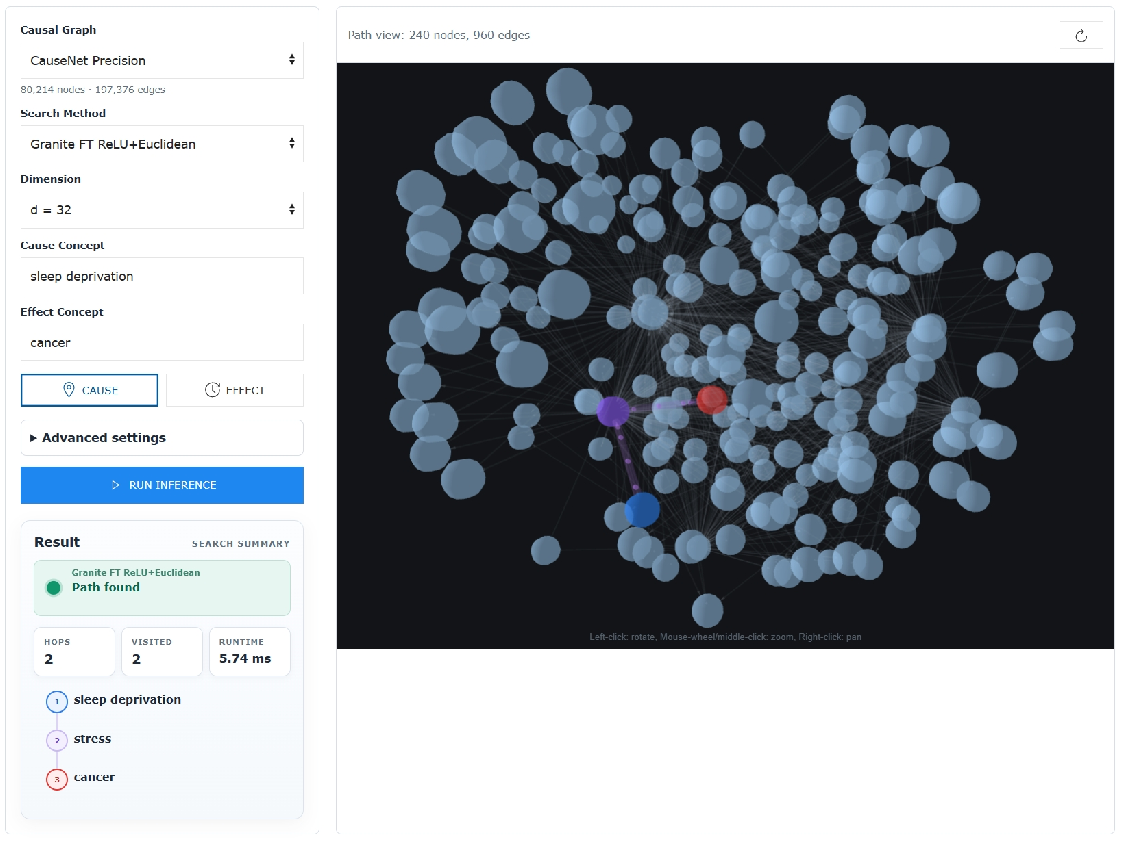
\includegraphics[width=\textwidth]{figures/app.pdf}
    \caption{Web interface for configuring embedding-guided $A^*$ search and visualizing the resulting causal path.}
    \label{fig:frontend-demo}
\end{figure}